\documentclass[10pt,twoside]{report}

\usepackage[utf8]{inputenc}
\usepackage[T1,T2A]{fontenc}
\usepackage[english,russian]{babel}
\usepackage[a6paper,top=1cm,bottom=1.5cm,left=1cm,right=1cm]{geometry}
\usepackage[inline]{enumitem}
\usepackage{graphicx}
\usepackage{float}
\usepackage{pbox}

\setdescription{labelindent=1cm, leftmargin=\parindent}

\begin{document}
% Title, illustration, name, band
\thispagestyle{empty}
\begin{center}
{\LARGE \textbf{Волот}}

\begin{figure}[H]
  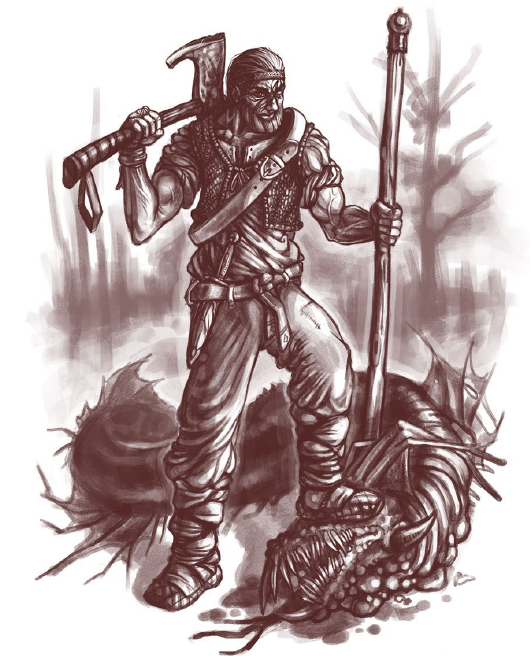
\includegraphics[width=170px]{images/volat.png}
\end{figure}

\end{center}
\begin{description}
\item[Имя:]\hfill
\item[Отряд:]\hfill
\end{description}
\pagebreak

%Description, guidelines
{\slshapeВолот}
\begin{itemize}[noitemsep]
  \item 
  \item 
  \item 
  \item 
\end{itemize}
\pagebreak

% Character info

\section*{Информация}
\begin{description}
\item[Имя]{\footnotesize (см. Имена и черты)}
\item[Внешность] {\footnotesize (Выбери несколько) Изнуренное лицо,
    безумные глаза,  вздутые вены, роба в бурых пятнах, длинные черные
    ногти, причудливый   плащ с капюшоном, кривые зубы\ldots}

\item[Черты характера]{\footnotesize (Выбери две, см. Имена и черты)}

\item[Цель] {\footnotesize (Что тебя ведет? Что ты ищешь на болотах?)
    Секрет   могущества? Способ разорвать темную сделку?}

\item[Страсть]{\footnotesize (В чем твоя слабость?) Садизм? Маковый порошок?}

\item[Темная предыстория]{\footnotesize (Почему ты бежал на болота?)}

\item[Контакт] {\footnotesize (Кто ждет тебя в городе?) Старый друг? Ученик?}

\item[Связь с отрядом]{\footnotesize (Почему ты доверяешь другим?)}
\end{description}
\pagebreak

% Stats

\section*{Характеристики}

\begin{center}
  \begin{tabular}{l c}
     Уровень & \verb!        !\\ 
  \end{tabular}

\begin{tabular}{|l|c|c|c|c|c|c|c|c|c|c|}
  \hline
  Опыт & & & & & & & & & &\\ \hline
\end{tabular}

{\footnotesize 10 опыта= новый уровень}
\end{center}
\begin{tabular}{l c}
  Cудьба{\tiny(Макс. 3)} & \\
  Козырь & \\
  Эссенции & \\ 
\end{tabular}

\begin{center}
\begin{tabular}{|p{2cm}|p{1cm}|p{1cm}|p{3cm}|}
\hline
  Распредели 7,5,4,2 & Макс & Текущ. & Ходы \\ \hline
  Стать & & & {\footnotesize Схватка, Запугивание}\\ [5ex] \hline
  Прыть & & & {\footnotesize Незаметность, Разведка, Скрытая Атака}\\ \hline
  Нрав & & & {\footnotesize Обман, Переговоры, При Смерти}\\ [5ex] \hline
  Ум & & & {\footnotesize Знания, Восприятие, Поиск Пути, Первая Помощь} \\ \hline
\end{tabular}

\begin{tabular}{|p{1.5cm}|p{1.5cm}|p{1cm}|p{3cm}|}
  \hline
   & Макс & Текущ. & Состояние \\ \hline
  Жизнь & 4+Стать & & Ранен($\leq 5$) \\ \hline
  Воля & 2+Нрав & & Сломлен($\leq 3$) \\ \hline
  Тьма & 10  & &  Осквернен($\geq 6$) \\ \hline
\end{tabular}

\end{center}

\pagebreak

% Inventory.

\section*{Инвентарь}

Твоя ноша = 5+Стать(\verb!   !). Ты {\scshape Перегружен}, если вес
предметов больше
\begin{center}
  {\footnotesize
\begin{tabular}{|p{2cm}|p{0.5cm}|p{4.5cm}|}
  \hline
  Название & Вес & Свойства \\ \hline
  Запасы {\tiny Макс. 10} & 2 & 5 запасов = Вес 1 \\
  Провиант & 1 & 5 рационов = Вес 1 \\
  Дукаты & 0 & 10 дукатов = Вес 1 \\ \hline
  Фолиант & 1 & В нем записаны все твои заклятья \\
  Ритуальный нож & 0 & 1р, урон 3, стать/прыть, вплотную, скрытое, зачарованный \\
  Зловещий плащ & 1 & Легкий доспех, броня 1, проблемный(заметный) \\
  Древний жезл & 2 & 1р, урон 4, стать, рядом, оглушение, статусный(культы) \\
   & & \\ [45ex]
   \hline  
\end{tabular}
}
\end{center}
\pagebreak


% Skills
\section*{Начальные ходы}
\begin{description}[noitemsep]
\item[Силач]--- Когда испытываешь Стать, совершая нечеловеческое
  усилие (поднимаешь валун, выбиваешь железную дверь\ldots),
  {\bfseriesпотрать 1 Волю}, чтобы игнорировать штрафы за Сложный
  ход.

  Вдобавок в бою {\bfseriesпотрать 1 Волю}, чтобы до конца сцены
  использовать любые топоры, копья, дубины или булавы как метательное
  оружие с параметрами: урон и бб такие же, как в ближнем бою,
  недалеко, стать, одноразовое. Если оружие осталось цело, то ты
  можешь его подобрать и снова использовать. Ты умеешь метать подобным
  образом тяжелые предметы (валуны, коряги\ldots)--- считай их оружием
  со свойствами: урон 3, недалеко, мощное, одноразовое.
  
  \vfill
  
  \item[Тутейший]--- Селяне и Болотные братья хорошо тебя знают и
  уважают. Считай, что у тебя всегда есть соответствующий статусный
  предмет. Также ты получаешь \textbf{бонус} на ход Знания, когда
  используешь его, чтобы установить факты о болотных тварях, местных
  жителях и их обычаях.

\vfill
  
  \pagebreak
  
\item[Клык цмока (ход на привале)]--- У тебя есть волшебный
  амулет. Когда ты убиваешь грозное или легендарное чудовище, ты
  можешь заключить его дух в свой амулет (может содержать не более 3
  духов чудовищ). В начале игры в амулет уже заключен один дух
  чудовища (опиши, кого ты убил недавно).

  В любое время сделай ход {\scshapeТьма сгущается}, чтобы при 3+
  выпустить один дух из амулета и получить один эффект (опиши его, он
  действует до конца сцены): 
  \begin{itemize}
  \itemКрепкая чешуя: Броня 3.
  \itemГибельная мощь: зачарованный и +1 к урону.
  \itemШипы и когти: оружие: урон 5, бб1, рядом, мощное.
  \itemГлаза смерти: Возможность видеть в темноте и бонус к Восприятию.
  \itemКожа-хамелеон: Бонус к Незаметности и Разведке.
  \itemЦепкие лапы: дает возможность ползать по любым твердым поверхностям.
  \end{itemize}

\pagebreak

\item[Убийца чудовищ]--- Пока ты сражаешься в легком доспехе или без
  брони, ты считаешь штраф за {\scshapeРазмер имеет значение} на 1
  меньше (этот ход сочетается с оружием со свойством Древковое).

  Убив грозное или легендарное чудовище, ты {\bfseriesвосстанавливаешь
    1 Волю}. Наконец, убив легендарное чудовище, наводящее ужас на
  округу, и добыв с него трофей (шкуру, голову, лапу\ldots--- вес 2),
  ты можешь получить за него награду (\textbf{3d6 дукатов}, монетами
  или услугами) у местных селян, купцов или шляхты.

  
\end{description}

\pagebreak

\section*{Новые ходы}
\begin{description}
\item[Кровавая ярость]--- Получи {\bfseriesбонус на боевые ходы}, пока Ранен.
\item[Сжав зубы (1 раз за сцену)]--- можешь {\bfseriesпотратить 1 Волю} вместо
  травмы.
\item[Житель болот (ход в лагере)]--- Твоя {\bfseriesНоша
    увеличивается на 1}. Также ты {\bfseriesполучаешь на 2 рациона
    больше}, когда успешно {\scshapeДобываешь продовольствие} или
  разделываешь съедобное чудовище.
\item[Сразись со мной! (1 раз за день)]--- Ты можешь вызвать грозное
  чудовище на ритуальный поединок: оно воспримет тебя как равного
  себе. {\bfseriesВыпусти один дух чудовища из своего амулета} и
  {\bfseriesиспытай Нрав}: \textbf{6+}:Ты одолел чудовище--- оно или в
  панике убежит, оставив тебе свое логово и добычу, или сделает то,
  что ты прикажешь (простая команда). \textbf{3-5}: Как 6+, но Мастер
  сделает ход. \textbf{1-2}: Ты проиграл. Мастер сделает ход.
\item[Мать сыра земля]--- когда ты сражаешься с противником лицом к лицу и пока стоишь ногами на твердой земле, ты {\bfseriesигнорируешь свойство {\scshapeМощное}} у атак противника (включая заклятья) и {\bfseriesполучаешь +1 Брони}.
\end{description}
\pagebreak

\section*{Темный ход}
\begin{description}
\item[Болотный цмок]--- твой амулет впитал так много сил чудовищ, что
  ты сам стал чудовищем. Отныне ты мерзкий болотный цмок под личиной
  человека: у тебя глаза и язык змея, из кожи проступает чешуя, тебя
  терзает жажда золота\ldots ( свойство {\scshapeПроблемное}). Твой
  метаболизм ускорился - ты всегда {\bfseriesпотребляешь на 1 рацион
    больше}, но и Восстанавливаешь Жизнь в двойном объеме. В полночь
  ты можешь {\bfseriesпотратить 1 Волю} и провести обряд, чтобы
  заключить в твой амулет дух чудовища из-за завесы (тебе не нужно
  никого убивать). Также тебе доступны новые эффекты для
  {\scshapeКлыка цмока}:
  \begin{itemize}[noitemsep]
  \itemКожаные крылья: дает возможность летать.
  \itemДыхание смерти: оружие: урон 3, бб5, зона, недалеко.
  \end{itemize}
 Кроме того, ты можешь  вместо одного выпустить два (три) духа чудовищ из своего амулета
    и использовать столько же эффектов. Вдобавок, если ты выпустишь 2
    духа (вместо 1), то можешь сделать ход Сразись со мной даже против легендарного чудовища. Однако отныне, пока действует эффект
    амулета, ты сбрасываешь личину и являешь свою истинную форму--- смешай свой человеческий облик и облик чудовища, чьи силы ты
    используешь (опиши). В этой форме ты также имеешь большой размер (см. Размер имеет значение).
 \item[Тьма возвращается]: твой амулет цел.
 \end{description}
 \vfill
\pagebreak
\end{document}
